\documentclass[11pt,a4paper]{article}
\usepackage[left=2cm,text={17cm,24cm},top=3cm]{geometry}
\usepackage[T1]{fontenc}
\usepackage[czech]{babel}
\usepackage[utf8]{inputenc}
\usepackage{url}
\usepackage{graphicx}
\usepackage{pdfpages}
\graphicspath{ {img/} }

\begin{document}

\begin{center}
\LARGE{Administrátorské rozhraní pro CMS}
\end{center}
Číslo projektu: 1\\
Číslo a název týmu: 139. Tým xstehl14\\
Autor: Petr Stehlík (xstehl14) \\
Další členové týmu: Mário Kuka (xkukam00), Martin Veis (xveism00)\\
Termín řešení: 21. 9. - 18. 12. 2015\\


\section*{Abstrakt}
Administrátorská webová rozhraní trpí mnoha UX prohřešky. Majoritní většina je nepřátelská, nepomáhající a zmatečná. Je zde několik důvodů proč tomu tak je. Administrátoři jsou minoritní skupina uživatelů dané stránky, negenerují přímý zisk, ale zprostředkovaný, a v neposlední řadě u administrátorů je velká motivace dosáhnout cíle (většinou je jejich prací udělat na webu X a Y a pokud tuto práci neodvedou, nadřízený nebude spokojen).

Největším problém současných administrátorských rozhraní je naprostá oddělenost od uživatelské části. Administrátor se musí přihlásit na speciální stránce (každý systém má adresu této stránky jinou) a přes tu vstoupit do administrace. Na e-shopech, při editaci produktu, zde nejdříve musí vyhledat správnou část administrace, správnou kategorii, v horším případě vyhledat rovnou produkt mezi tisíci dalších a objeví se obrovský formulář pro editaci produktu.

S nastupujícími moderními technologiemi tento problém nemusí být až tak velký. Proto jsme se rozhodli navrhnout administrátorské rozhraní, které nebude až tak administrátorské jako spíše uživatelské. Administrátor nebude mít vlastní stránky na editaci, ale bude mít k dispozici editační mód přímo na stránce, kterou návštěvník vidí a použivá. Tím odpadá obrovská režie pro administrátora, který nemusí odhadovat, co uživatel uvidí, jak se změna projeví, atp. Své úpravy uvidí přímo na dané stránce v daný okamžik a tím se přibližíme k plně funčnímu WYSIWYG editoru.

\section*{Cílové požadavky na aplikaci a její rozhraní}
Hlavním cílem našeho snažení je vytvořit plnohodnotý e-shop, který nebude mít administrační rozhraní oddělené od uživatelského. Toho docílíme editačním módem uvnitř e-shopu. Aplikace tím pádem nemusí obhospodařovat dva, technicky vzato, rozdílné weby, ale vše obstará \uv{front-end} pro uživatele.

Odstraněním \uv{back-endu} dosáhneme rychlejší a smysluplné editace stránek. Administrátor není nucen přecházet mezi 2 stránkami a načítat celý obsah znovu. Jakoukoliv úpravu ihned vidí. To odstraňuje další problém rezonující napříč všemi e-shopy -- nevydařené úpravy. Uživatel nemůže přijít na e-shop, který je zrovna v údržbě.


\section*{Studium uživatelů, UI a testování}
Díky velmi specifické cílové skupině, pro kterou navrhujeme, jsou zde určitá omezení. Nemůžeme použít nepřesné nebo zavádějící názvy akcí. Na druhou stranu máme velmi motivovanou cílovou skupinu, která má jasné cíle. Touto problematikou se zajímá několik projektů, většina z nich je ale pouhým rozšířením stávajících CMS. Např. pro Wordpress existuje rozšíření Cornerstone\footnote{\url{http://www.liveeditorcms.com/}} nebo pro OpenCart Live Theme Editor\footnote{\url{http://www.opencart.com/index.php?route=extension/extension/info&extension_id=20693}}.

Nejefektivnější a nejvíce vypovídající metodologií testování je testování s reálnými uživateli. Např. A/B testování není v tuto chvíli proveditelné, protože nemáme zavedený eshop, na kterém bychom mohli testovat, navíc se jedná o kompletně nový CMS s vlastním databázovým schématem.


\section*{Návrh GUI}
Nejdůležitější funkčností aplikace je živá editace obsahu. Úpravy, které administrátor provede, okamžitě uvidí a může se tak rychle rozhodnout, zda úpravy, které provedl, jsou vhodné. Tímto způsobem může administrátor upravit jakoukoliv část webu a jeho obsahu, logem počínaje, patičkou konče.

Při návrhu GUI je vhodné používat interaktivní wireframe, protože v případě statických wireframe nedokážeme demonstrovat celkovou dynamičnost aplikace. Prvotní návrhy probíhají na papíře a ty přímo přetváříme do low-fidelity wireframe (viz Přílohy). Ten se následně vylepší a s dodanou funkcionalitou vytvoříme high-fidelity wireframe.

Po průzkumu současných e-shop CMS jsme zhodnotili, že tento typ rozhraní v současné chvíli neexistuje, případně jako pouhé pokusy. To s sebou nese řadu nevýhod, které ale eliminujeme nástroji odzkoušenými v praxi a zkušenostmi v oboru.

%%%%%%%%%%\Large{Připravte mockupy rozhraní}

\section*{Návrh testování}
Z hlediska povahy aplikace a jejího zaměření budeme provádět kvalitativní testování na několika typech uživatelů, kteří se s aplikací mohou dostat do styku. S ohledem na neveřejnost projektu by navíc bylo velmi těžké vytvořit kvantitativní testování.
\begin{enumerate}
	\item{Počítačově zkušení uživatelé (programátoři)}
	\item{Správci e-shopů}
	\item{Pokročilejší uživatelé PC}
	\item{Běžní uživatelé PC}
	\item{Počítačově negramotní uživatelé}
\end{enumerate}

Nejdůležitějšími skupinami uživatelů jsou číslo 2 a 3, kteří jsou nejpravděpodobnější uživatelé této aplikace. 

\section*{Studium realizace GUI}
Z hlediska povahy projektu je nejvhodnější webové řešení. Je zde i možnost desktopového řešení, ale tím by celý návrh ztratil smysl v podobě odděléno back-endu. Webové řešení má navíc několik výhod. Je velmi lehce přenositelné, dostupné kdekoliv (i na mobilních zařízeních) a nezávislé na platformě.

Nevýhodou webového řešení je částečně různá interpretace aplikace na webových jádrech prohlížečů. Tyto rozdíly jsem ale víceméně kosmetické a neubírají aplikaci na funkcionalitě.

Konkrétně pro front-end jsme vybrali velmi silnou kombinaci HTML 5 a CSS3 pro zobrazování a AngularJS\footnote{\url{https://angularjs.org/}} pro obsluhu front-endu. AngularJS je javascriptový MVC framework pro dynamickou manipulaci s webovou stránkou (two-way data binding). Zároveň slouží jako server pro celou stránku (z hlediska front-endu).

Pro serverový back-end jsme zvolili jazyk Python a knihovnu Flask\footnote{\url{http://flask.pocoo.org/}}. Back-end slouží pouze pro komunikaci s databází a kontrolu uživatelů (udržování session). Knihovna Flask je použita pro tvorbu webového API, aby mohl front-end komunikovat s back-endem. 

Python oproti PHP disponuje excelentní vyjadřovací schopností, je efektivnější a jednodušší k použití. Společně s různými knihovnami se tyto schopnosti ještě více umocňují.
% Jaké technologie jsou vhodné pro řešení aplikace a UI?
% Čím je vhodná vybraná technologie (Qt, WPF, web tech. apod.)? Co přináší a v čem je naopak takovéto řešení omezující?
% Jaké specifické části technologie (popř. rozšiřujících nástrojů) jsou pro řešení vybrány a proč?
% Sepište do TZ.

\section*{Návrh back-endu}
Pro plnou funkčnost aplikace je potřeba webový server s veřejnou IP adresou, v našem případě Linuxový server s Apache, databáze MySQL a jazyk Python s knihovnou Flask. Apache je konfigurován na spouštění WSGI skriptů (Python). 

Struktura celé aplikace je znázorněna na schématu, které ukazuje i použité technologie.
\newline
\newline
\centerline{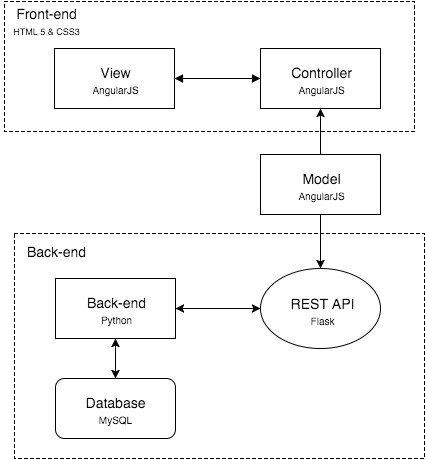
\includegraphics[scale=0.5]{schema.png}}

% Jaké služby/funkce (server, datový model, sada funkcí, služby třetích stran apod.) je třeba připravit pro dostatečnou funkčnost a testování GUI aplikace? 
% Funkce nemusí být funkční (dynamické apod.), ale musí vracet smysluplné hodnoty (simulované hodnoty, pevně přednastavené ...).
% Jaká je struktura aplikace a napojení GUI na back-end?
% Zpracujte do TZ.

\section*{Programování back-endu}
Back-end je, jak zmíněno výše, realizován v jazyku Python společně s knihovnou Flask. Ten obsluhuje veškerou práci s databází dle požadavků od front-endu.

Databázové schéma bylo převzato z dřívějšího projektu do předmětu IDS z druhého ročníku. Toto schéma jsme upravili a rozšířili. Částečné schéma je níže v přílohách.

% Programování back-endu
% Naprogramujte a připravte na použití. 
% Klíčové informace o back-endu (stručný popis, struktura programového řešení, vybrané funkce, API) popište v TZ.
% Toto nemusí dělat všichni členové týmu.


% Co jsou klíčové prvky GUI realizující cíle aplikace?\\
% Jak se pozná, že jsou efektivní?\\
% Na jakém vzorku uživatelů proběhne testování?\\
% Jakým způsobem bude probíhat testování, aby mělo dostatečnou vypovídající hodnotu (s ohledem na omezený počet testovacích uživatelů)?\\
% Jaké úlohy budou testeři řešit? Jaký vliv má pořadí a složitost úloh na výsledky testování?\\
% Připravte testovací protokol. Přiložte k TZ jako přílohu. 

\section*{Přílohy}

\subsection*{Návrh rozhraní -- běžný uživatel}
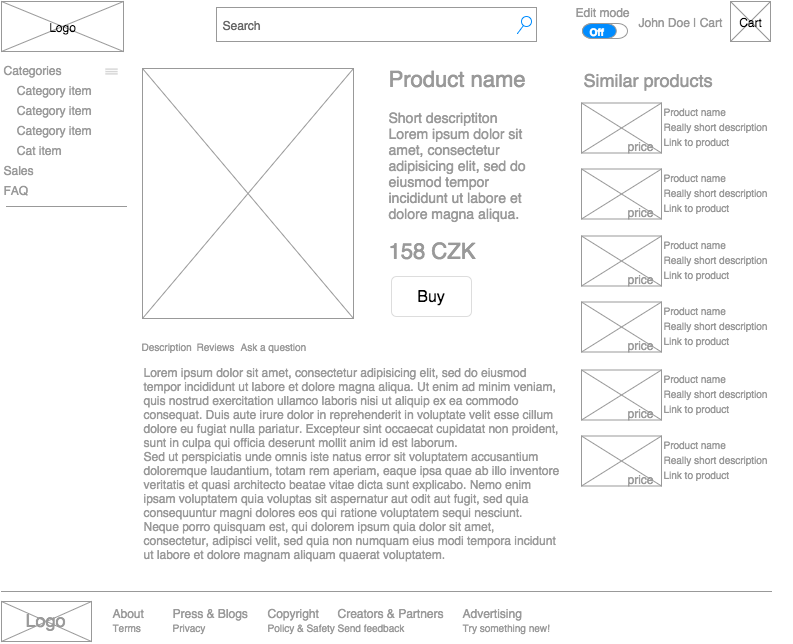
\includegraphics[scale=0.6]{pyngshop.png}
\subsection*{Návrh rozhraní -- administrátor}
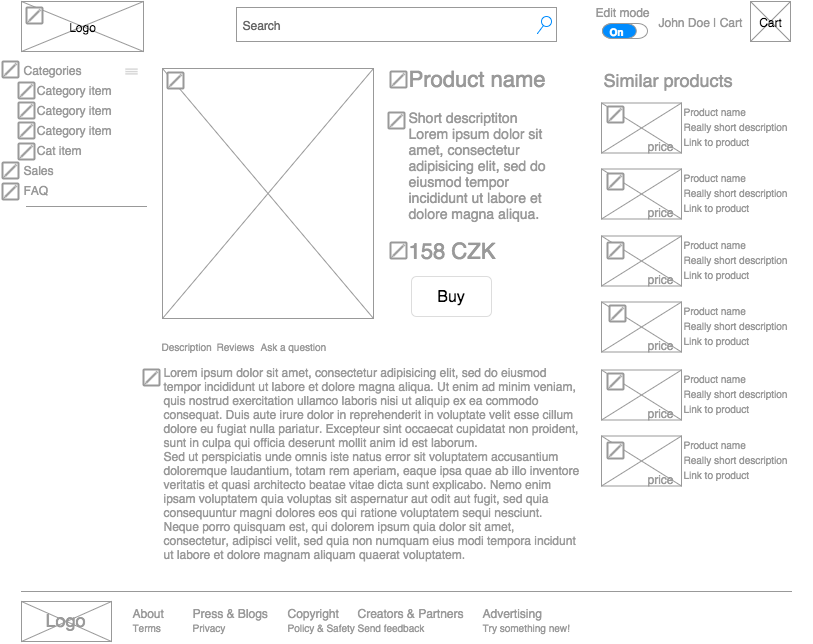
\includegraphics[scale=0.6]{pyngshop_edit.png}
\newpage

\subsection*{Databázové schéma}
\centerline{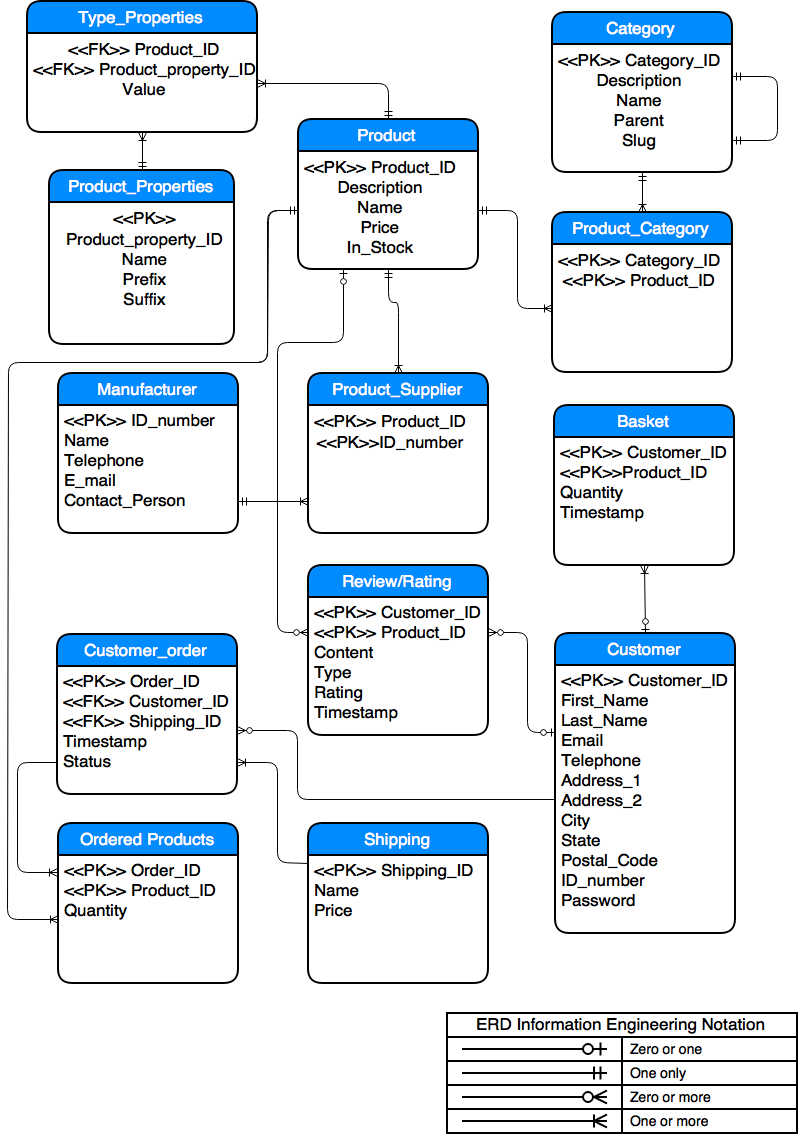
\includegraphics[scale=0.55]{eshop_erd.png}}
\newpage

\subsection*{Testovací protokol}
\noindent{\large\textsc{Úkol}: Vytvořte nový produkt v kategorii XYZ.}\\
\textsc{Cíl}: Vytvoření produktu v dané kategorii.\\
\textsc{Čas}: 5 minut s připravenými podklady.\\
\bigskip

\noindent{\large\textsc{Úkol}: Upravte produkt ABC v kategorii XYZ.}\\
\textsc{Cíl}: Upravení produktu v dané kategorii.\\
\textsc{Čas}: 2 minuty pro minoritní úpravu.\\
\bigskip

\noindent{\large\textsc{Úkol}: Vyřiďte příchozí objednávky (vytisknout faktury).}\\
\textsc{Cíl}: Vytištění faktur do PDF a uložení.\\
\textsc{Čas}: 3 minuty do finálního uložení všech faktur.\\
\bigskip

\noindent{\large\textsc{Úkol}: Upravte název kategorie A na B.}\\
\textsc{Cíl}: Upravení názvu zanořené kategorie.\\
\textsc{Čas}: 1 minuta.\\
\bigskip

\noindent Ke každému úkolu zaznamenáváme čas provedení, komplikace při provádění, otázky uživatele, úroveň frustrace vykonavatele, úroveň zmatení a spokojenost s výsledkem
\end{document}